\section{Auswertung}
\label{sec:Auswertung}

\subsection{statische Messung}
\label{subsec:stat}

T1 Messing dick fern
T2 Messing dick nah
T3 Messing dünn nah 
T4 Messing dünn fern
T5 Aluminium fern
T6 Aluminium nah
T7 Edelstahl nah
T8 Edelstahl fern

\begin{figure}[!htbp]
  \centering
  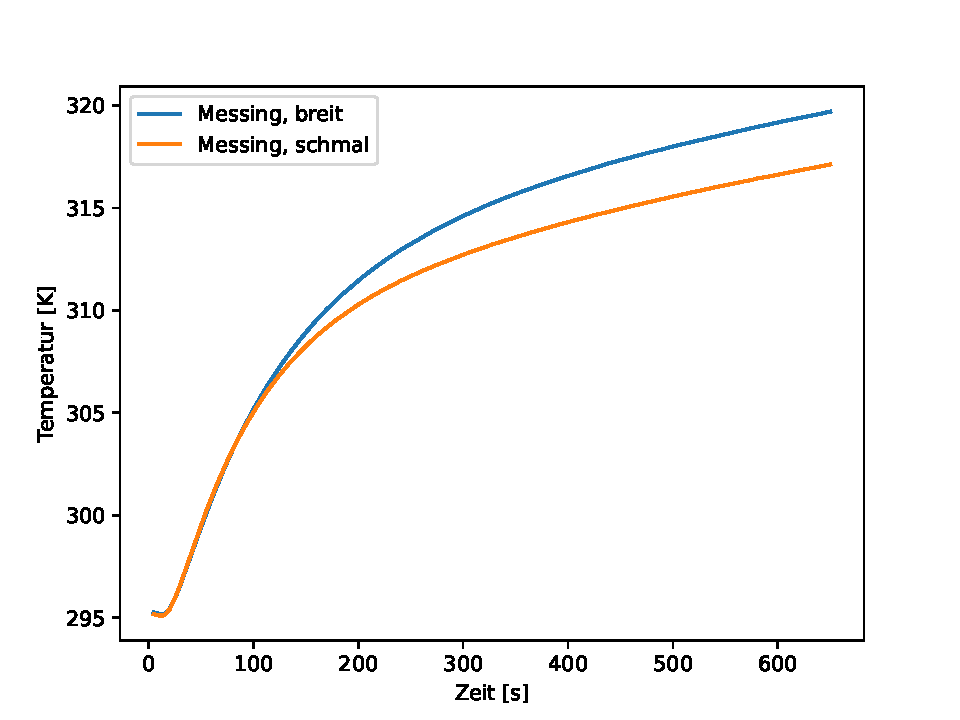
\includegraphics{verlauf_mess.pdf}
  \caption{Temperaturverlauf der Messingstäbe (fern)}
  \label{fig:mess}
\end{figure}

\begin{figure}[!htbp]
  \centering
  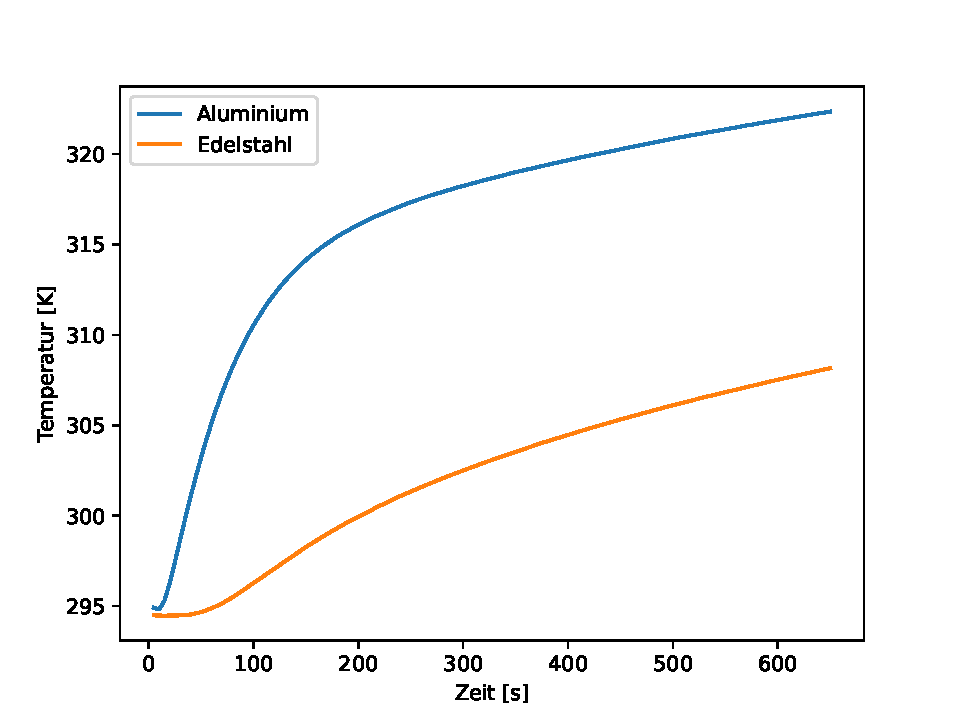
\includegraphics{verlauf_alu_edel.pdf}
  \caption{Temperaturverlauf des Aluminium- und Edelstahlstabs (fern)}
  \label{fig:alu_edel}
\end{figure}

\begin{figure}[!htbp]
  \centering
  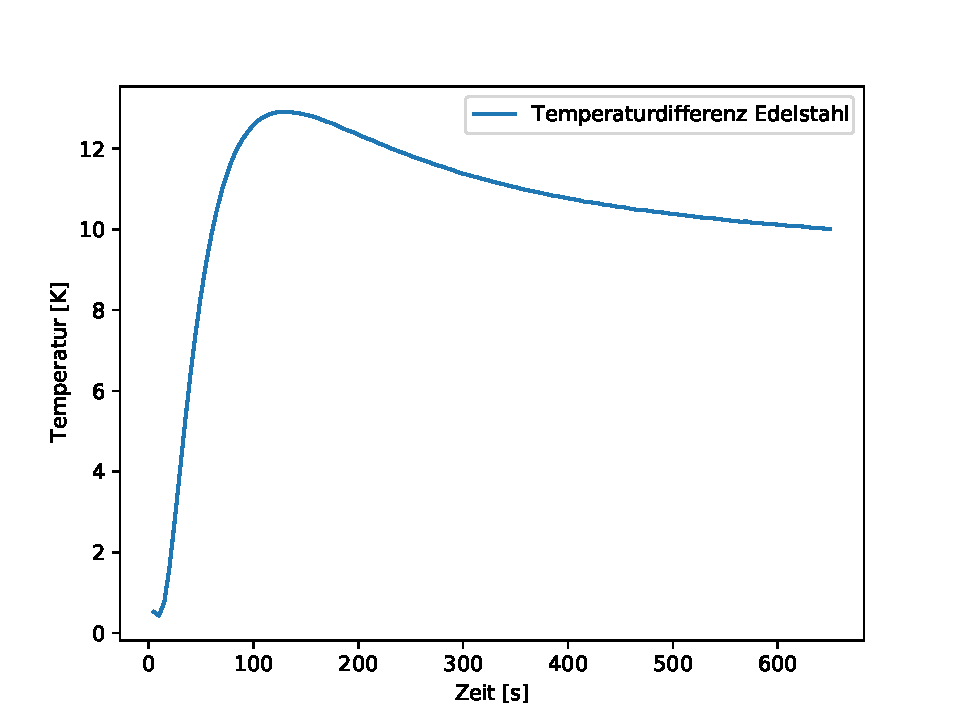
\includegraphics{differenz_edel.pdf}
  \caption{Verlauf der Temperaturdifferenz am Edelstahlstab}
  \label{fig:diff_edel}
\end{figure}

\begin{figure}[!htbp]
  \centering
  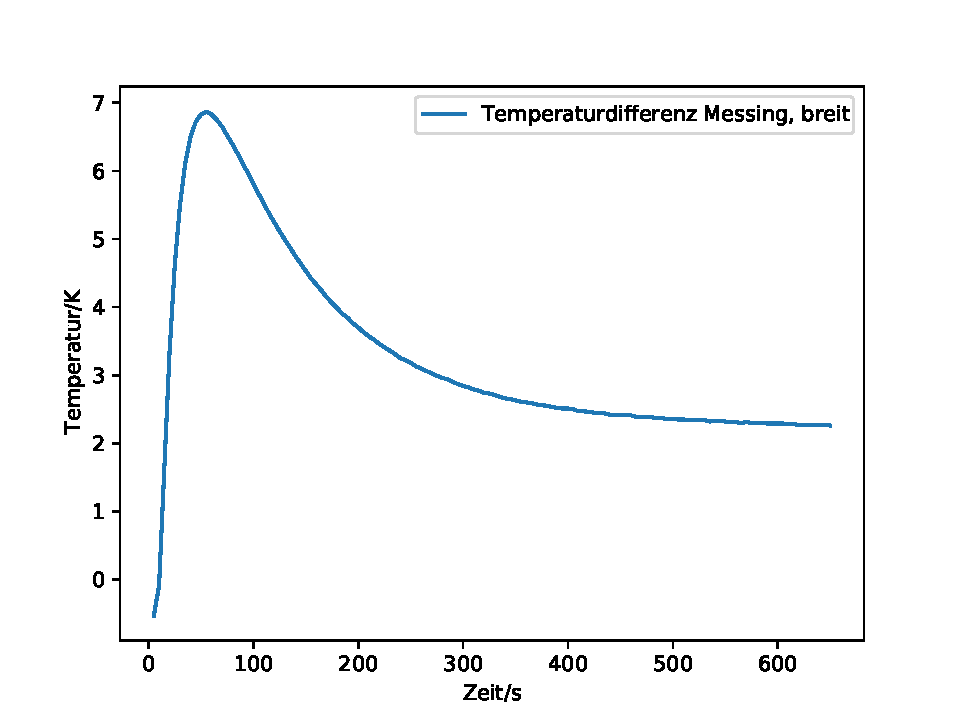
\includegraphics{differenz_mess.pdf}
  \caption{Verlauf der Temperaturdifferenz am breiten Messingstab}
  \label{fig:diff_mess}
\end{figure}

\begin{figure}[!htbp]
  \centering
  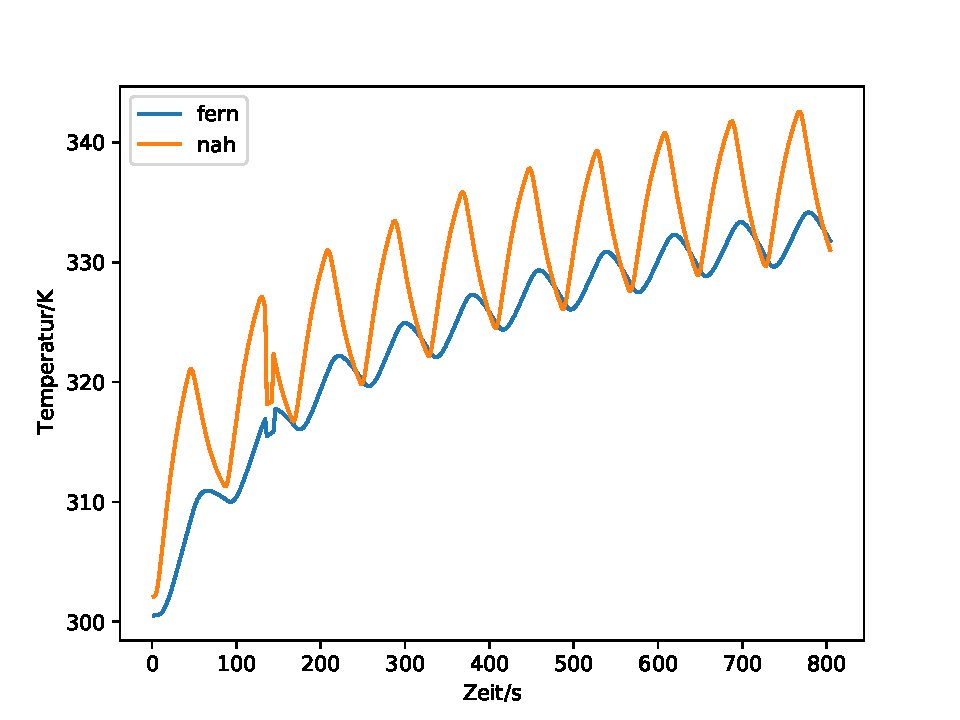
\includegraphics{dyn_80_mess.pdf}
  \caption{Temperaturverlauf des breiten Messingstabs}
  \label{fig:mess_dyn}
\end{figure}

\begin{figure}[!htbp]
  \centering
  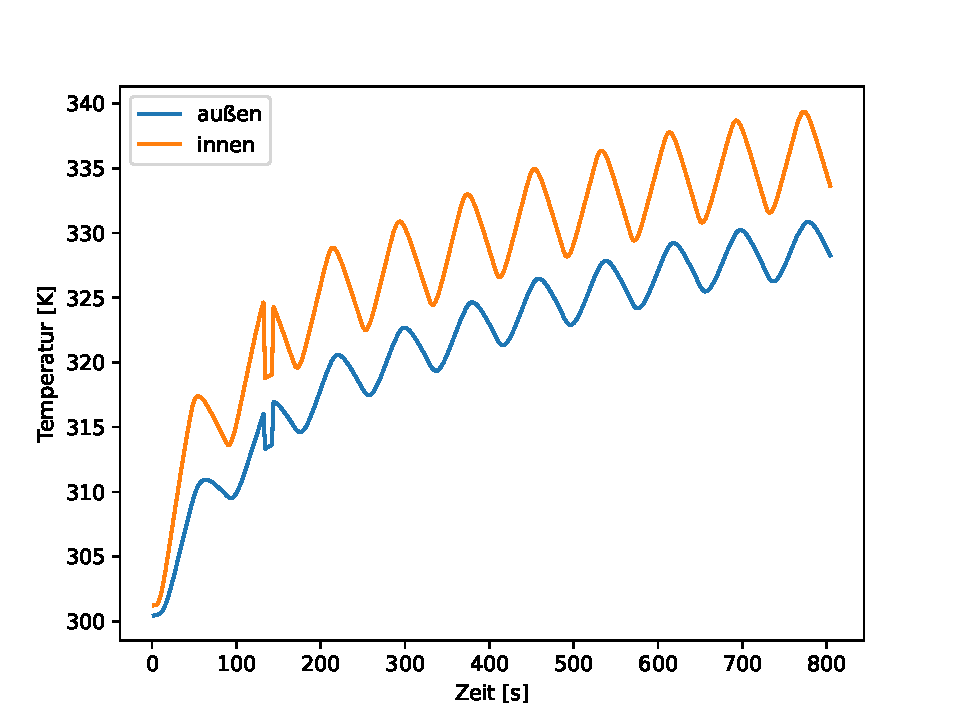
\includegraphics{dyn_80_alu.pdf}
  \caption{Temperaturverlauf des Aluminiumstabs}
  \label{fig:alu_dyn}
\end{figure}

\begin{figure}[!htbp]
  \centering
  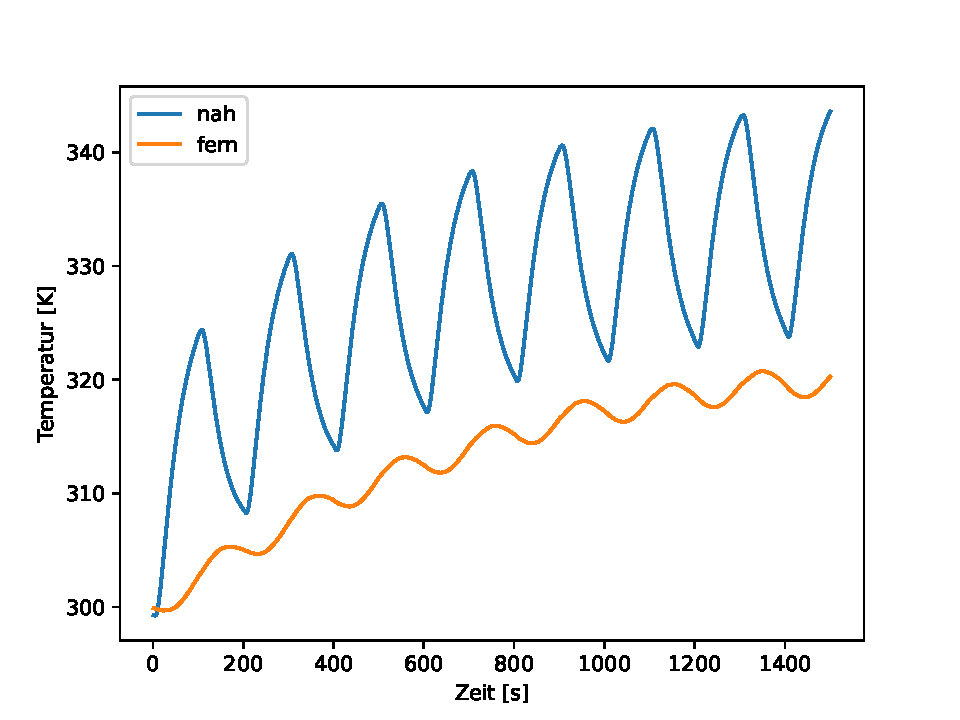
\includegraphics{dyn_2.pdf}
  \caption{Temperaturverlauf des Edelstahlstabs}
  \label{fig:edel_dyn}
\end{figure}



